\documentclass[border=6pt]{standalone}
\usepackage{amsmath}
\usepackage{tikz}
\usetikzlibrary{arrows.meta}
\begin{document}
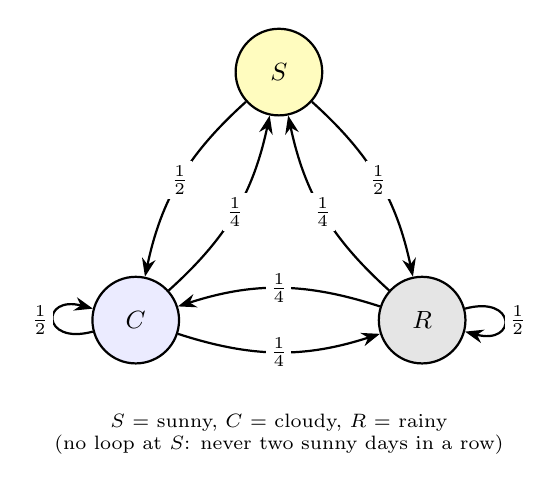
\begin{tikzpicture}[>=Stealth,font=\small,
 s/.style={draw,thick,circle,minimum size=1.1cm,inner sep=0pt,fill=blue!8},
 e/.style={->,thick},
 lab/.style={font=\small,fill=white,inner sep=1.5pt},
 every loop/.style={->,thick,looseness=6}]
\node[s,fill=yellow!25] (S) at (90:2.1) {$S$};
\node[s] (C) at (210:2.1) {$C$};
\node[s,fill=gray!20] (R) at (-30:2.1) {$R$};
\draw[e] (S) to[bend right=18] node[lab]{$\tfrac12$} (C);
\draw[e] (C) to[bend right=18] node[lab]{$\tfrac14$} (S);
\draw[e] (S) to[bend left=18] node[lab]{$\tfrac12$} (R);
\draw[e] (R) to[bend left=18] node[lab]{$\tfrac14$} (S);
\draw[e] (C) to[bend right=18] node[lab]{$\tfrac14$} (R);
\draw[e] (R) to[bend right=18] node[lab]{$\tfrac14$} (C);
\path (C) edge[loop left] node[lab]{$\tfrac12$} (C);
\path (R) edge[loop right] node[lab]{$\tfrac12$} (R);
\node[font=\scriptsize,align=center] at (0,-2.5) {$S$ = sunny, $C$ = cloudy, $R$ = rainy\\(no loop at $S$: never two sunny days in a row)};
\end{tikzpicture}
\end{document}
